\chapter{Giới thiệu}
\label{Chapter1}

Việc sử dụng mạng nơ-ron nhiều tầng ẩn trong các ứng dụng trí tuệ nhân tạo ngày càng chiếm một vị trí quan trọng khi mà các bài toán khó của học máy truyền thống trong xử lý ảnh và video, xử lý ngôn ngữ tự nhiên như: dịch máy tự động, nhận diện mặt người, phát hiện đồ vật,... đã phần nào được giải quyết và ngày càng được cải tiến.

Mạng nơ-ron nhiều tầng ẩn là một mạng nơ-ron nhân tạo gồm ba loại tầng chính: tầng nhập, các tầng ẩn, và tầng xuất. Việc có nhiều tầng ẩn cũng là một trong những lý do giúp mạng nơ-ron nhiều tầng ẩn có thể giải quyết các bài toán khó mà các thuật toán học máy truyền thống không giải quyết được. Mặc dù vẫn còn nhiều ý kiến về việc sử dụng nhiều tầng ẩn có thực sự cần thiết như công trình của Jimmy Lei Ba\cite{ba2013dodeepnets} chứng minh được rằng một mạng nơ-ron nông (shallow network) vẫn có thể xấp xỉ kết quả của một mạng nơ-ron nhiều tầng ẩn. Tuy nhiên, để đạt được kết quả đó, bài báo phải sử dụng một tập dữ liệu có kích thước rất lớn và một mạng nơ-ron nhiều tầng ẩn có độ chính xác khá cao. Ngoài việc mạng nơ-ron nhiều tầng ẩn có thể giúp cho quá trình thiết kế mô hình cho từng bài toán dễ dàng hơn\cite{nielsen2015neural} thì sức mạnh rút trích đặc trưng tự động cũng đã được chỉ ra trong nhiều bài báo khác: Yoshua Bengio và Yann Lecun lý giải rằng với nhiều tầng ẩn, mạng nơ-ron có thể ``học'' được từ đặc trưng đơn giản (low-level features) và tạo thành các đặc trưng phức tạp hơn (higher-level features)\cite{bengio2007scaling}; một công trình khác của Yoshua Bengio cho thấy sức mạnh của mạng nơ-ron nhiều tầng ẩn khi nó có thể giải quyết các bài toán mà các mạng nơ-ron ít tầng ẩn hơn không thể\cite{bengio2009learning}.

\begin{figure}[htp]
\centering
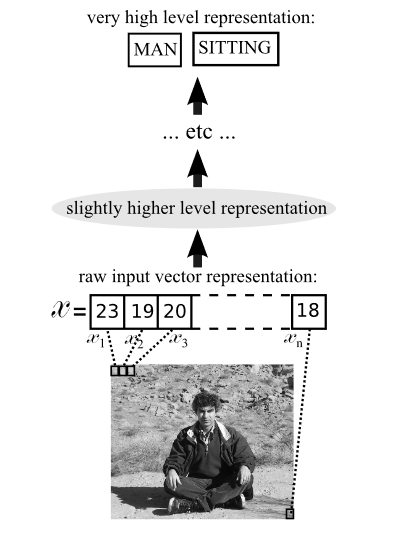
\includegraphics[width=65 mm]{images/layers-features.png}
\caption{Minh hoạ quá trình mạng nơ-ron ``học'' từ các đặc trưng đơn giản, như các điểm ảnh, tạo thành các đặc trưng phức tạp hơn.\cite{bengio2009learning}}
\label{fig:layers-features}
\end{figure}

Tuy nhiên, mặc dù mạng nơ-ron có càng nhiều tầng ẩn sẽ khiến cho độ chính xác trong tập huấn luyện ngày càng tăng nhưng độ chính xác trong tập kiểm thử ngày càng giảm. Đây là biểu hiện của việc mô hình bị overfit, đồng nghĩa với việc mô hình chỉ ``ghi nhớ'' tập huấn luyện nhưng không thể tổng quát hóa những đặc trưng đã học để tiến hành đưa ra dự đoán trên tập kiểm thử. Ngược lại, nếu mạng nơ-ron quá đơn giản, có thể có ít tầng ẩn hoặc mỗi tầng ẩn có số lượng nơ-ron ít, thì mô hình đó không đủ khả năng để rút trích ra những đặc trưng có ý nghĩa mà mô hình có thể học khiến cho độ chính xác ở cả hai tập dữ liệu huấn luyện và kiểm thử đều giảm (Hình \ref{fig:under-over}).

\begin{figure}[htp]
\centering
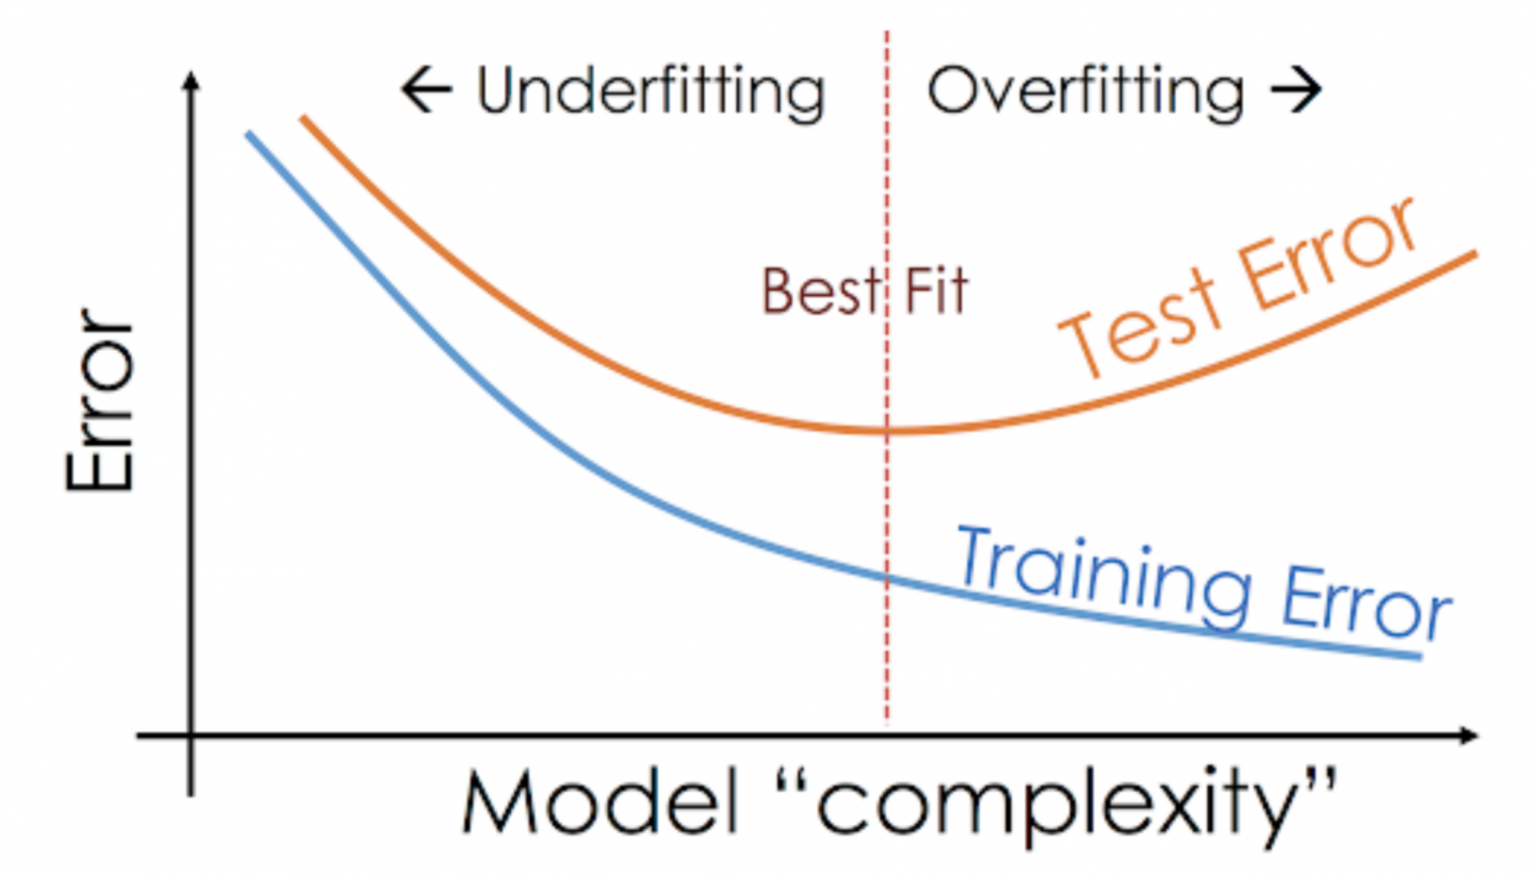
\includegraphics[width=100 mm]{images/under-over.png}
\caption{Minh họa cho mô hình overfit và underfit. (Nguồn: \url{https://www.analyticsvidhya.com/blog/2020/02/underfitting-overfitting-best-fitting-machine-learning})}
\label{fig:under-over}
\end{figure}

Một mạng nơ-ron nhiều tầng ẩn được xem là có khả năng tổng quát hoá tốt trên một bài toán khi sự sai khác giữa giá trị dự đoán của mạng nơ-ron và giá trị nhãn của dữ liệu ngoài tập huấn luyện là đủ nhỏ (trong bài toán huấn luyện có giám sát). Để đạt được kết quả đó, mạng nơ-ron nhiều tầng ẩn cần đi tìm một bộ trọng số phù hợp cho từng bài toán cụ thể. Việc đi tìm bộ trọng số này được thực hiện thông qua quá trình tối ưu hoá mạng nơ-ron nhiều tầng ẩn.

Bài toán tối ưu hoá mạng nơ-ron nhiều tầng ẩn nhận dữ liệu nhập là hàm chi phí nhận bộ trọng số của mạng nơ-ron nhiều tầng ẩn làm tham số. Hàm chi phí cho biết sự sai lệch giữa kết quả dự đoán của mạng nơ-ron so với giá trị đúng. Giá trị sai lệch này còn được gọi là độ lỗi. Sau quá trình tối ưu ta mong muốn có được một bộ trọng số của mạng nơ-ron nhiều tầng ẩn cho độ lỗi trong cả hai tập dữ liệu huấn luyện và tập dữ liệu kiểm tra là đủ nhỏ.

\begin{figure}[htp]
\centering
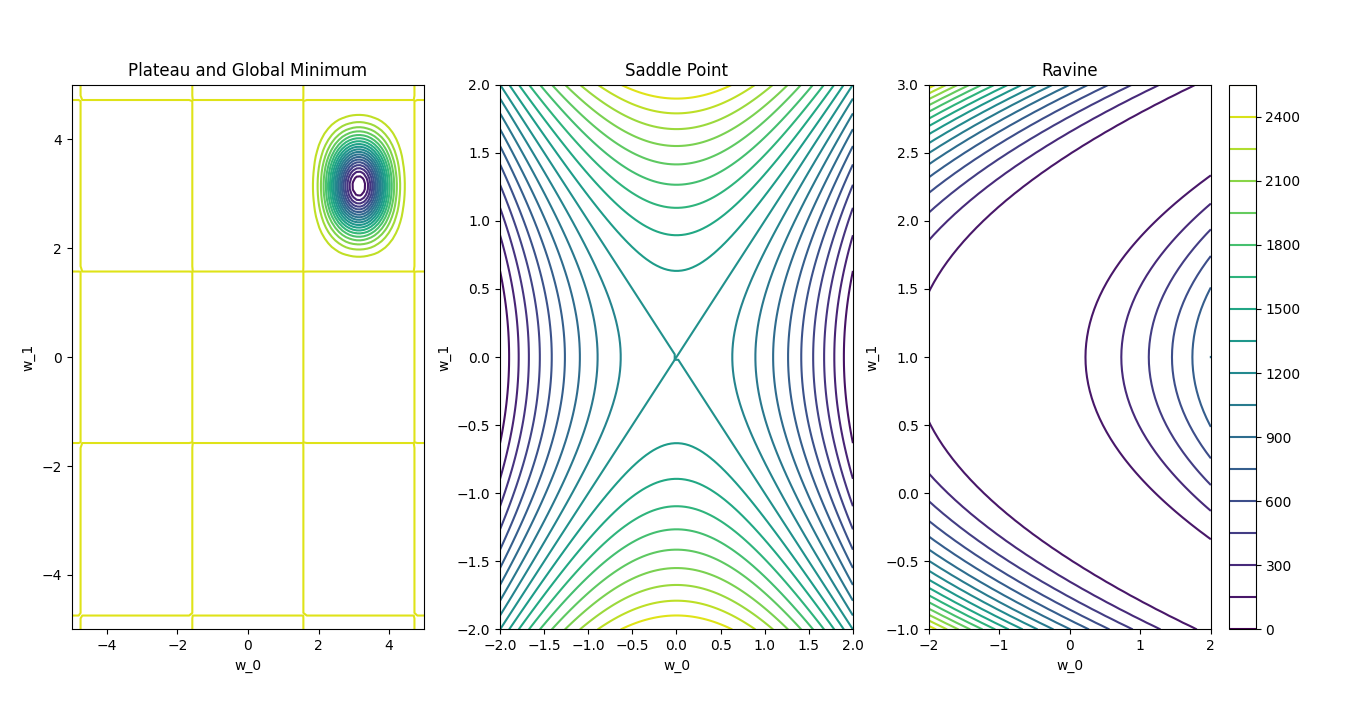
\includegraphics[width=120 mm]{images/cricial-point-contour.png}
\caption{Đồ thị contour cho những điểm critical point: vùng bằng phẳng có một cực tiểu (trái), điểm yên ngựa (giữa), vùng rãnh hẹp (phải).}
\label{fig:cricial-point-contour}
\end{figure}

Việc tối ưu hoá mạng nơ-ron có thể hiểu là quá trình đi tìm cực tiểu của hàm chi phí bằng cách thay đổi giá trị của bộ trọng số. Từ đó, ta cũng có thể hiểu quá trình tối ưu hoá mạng nơ-ron là quá trình di chuyển trong mặt phẳng lỗi (Hình \ref{fig:resnet-loss}) để tìm được tọa độ của một điểm trên mặt phẳng được định nghĩa bởi hàm lỗi cho giá trị độ lỗi là đủ nhỏ. Tuy nhiên, việc di chuyển trong mặt phẳng lỗi gặp nhiều khó khăn. Li Hao và cộng sự\cite{li2018visualizing} cho thấy rằng sự hỗn loạn của mặt phẳng lỗi ngày càng tăng khi số tầng ẩn trọng mạng nơ-ron ngày càng tăng. Sự hỗn loạn này được cấu thành từ nhiều ``critical point'' (Hình \ref{fig:cricial-point-contour}), những điểm có gradient bằng 0, như cực tiểu địa phương, điểm yên ngựa, hợp với các vùng bằng phẳng, và vùng rãnh hẹp.

\begin{figure}[htp]
\centering
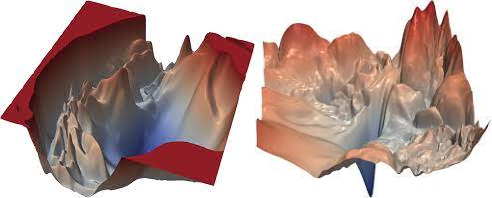
\includegraphics[width=120 mm]{images/resnet-loss.png}
\caption{Bề mặt lỗi của mô hình ResNet-110 (trái) và bề mặt lỗi của mô hình ResNet-56 (phải).\cite{li2018visualizing}}
\label{fig:resnet-loss}
\end{figure}

Các điểm cực tiểu địa phương từng được xem như là nguyên nhân chính gây ra sự khó khăn trong việc tối ưu hoá mạng nơ-ron có nhiều tầng ẩn, nhưng nghiên cứu của Quynh Nguyen và Matthias Hein\cite{nguyen2017thelosssurface} đã chỉ ra rằng việc đi tìm cực tiểu toàn cục thật sự có thể mất nhiều thời gian nhưng cho hiệu quả không đáng kể. Yann N. Dauphin cũng cho rằng khi số lượng tầng ẩn quá lớn thì tất cả các điểm critical point sẽ là điểm yên ngựa và các điểm cực tiểu tìm được đều có độ lỗi ngang với cực tiểu toàn cục. Hơn nữa, các điểm yên ngựa thường được bao bọc bởi một vùng gần như bằng phẳng, là vùng mà tại đó đạo hàm xấp xỉ gần bằng 0, làm chậm tốc độ của đa số các thuật toán tối ưu thường được sử dụng hiện nay. Vì thế, việc tránh và tìm được cách thoát ra khỏi điểm yên ngựa là quan trọng đối với các thuật toán tối ưu.

\begin{figure}[htp]
\centering
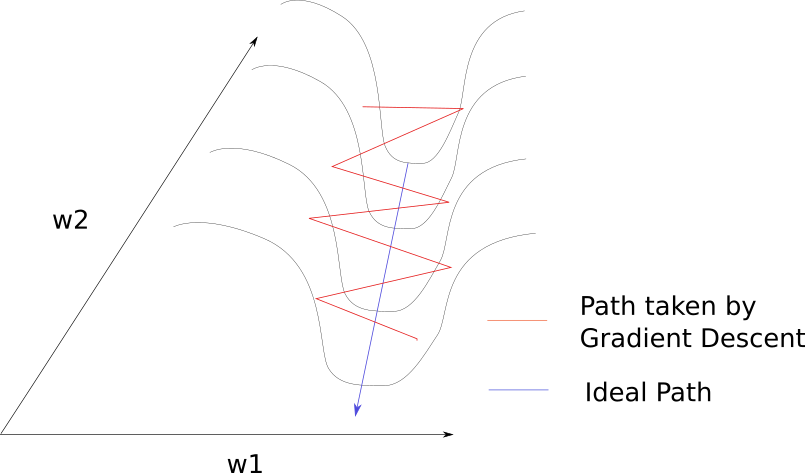
\includegraphics[width=100 mm]{images/valley.png}
\caption{Minh họa cho hướng đi của gradient trong trường hợp di chuyển trong rãnh hẹp. (Nguồn: \url{https://blog.paperspace.com/intro-to-optimization-momentum-rmsprop-adam/})}
\label{fig:valley}
\end{figure}

Ngoài các điểm yên ngựa, bề mặt lỗi còn đặc trưng bởi độ cong tại mỗi hướng, tương ứng với một trọng số của mạng nơ-ron nhiều tầng ẩn (Hình \ref{fig:valley}). Độ cong tại một hướng trên bề mặt lỗi cho ta biết tốc độ thay đổi gradient của hàm chi phí. Một hướng có độ cong thấp (low-curvature, như hướng $w_2$ trong hình) đồng nghĩa với gradient sẽ ít thay đổi khi $w_2$ thay đổi và ngược lại, một hướng có độ cong cao (high-curvature, như hướng $w_1$ trong hình) sẽ cho giá trị gradient thay đổi nhiều khi giá trị $w_1$ thay đổi. Vùng được đồng thời tạo bởi các hướng có độ cong cao và độ cong thấp được gọi là vùng rãnh hẹp. Hiện tượng này xuất hiện thường xuyên trong mạng nơ-ron nhiều tầng ẩn do ảnh hưởng của mỗi trọng số lên độ lỗi là khác nhau và giá trị trọng số sẽ phụ thuộc vào giá trị trọng số ở các tầng trước đó. Một giải pháp thường được sử dụng để vượt qua các vùng này là lựa chọn một bước cập nhật đủ nhỏ để tránh dao động quanh hướng có độ cong cao nhưng vẫn đủ để tiếp tục di chuyển theo hướng có độ cong thấp về hướng cho độ lỗi thấp hơn. Tuy nhiên, cách giải quyết này cho thời gian huấn luyện quá chậm để có ý nghĩa thực tiễn.

Trong thời gian đầu, việc huấn luyện mạng nơ-ron nhiều tầng ẩn sử dụng các phương pháp bậc nhất, các phương pháp này chỉ sử dụng đạo hàm bậc nhất của bề mặt lỗi tại vị trí hiện tại. Việc sử dụng đạo hàm bậc nhất/gradient sẽ cho biết hướng có độ dốc lớn nhất của bề mặt lỗi tại một điểm. Do đó, các phương pháp bậc nhất thường chỉ thực hiện những bước cập nhật rất nhỏ theo hướng gradient để tránh trường hợp bị vượt qua khỏi những vùng thấp hơn có khả năng chứa cực tiểu của bề mặt lỗi. Các phương pháp bậc nhất thường không gặp vấn đề mắc kẹt tại điểm yên ngựa vì hướng của gradient luôn đảm bảo tìm thấy một điểm mới có độ lỗi nhỏ hơn điểm hiện tại (nếu điểm hiện tại không phải là critical point). Thế nhưng, chúng thường bị mắc kẹt tại các vùng bằng phẳng xung quanh điểm yên ngựa.

Việc sử dụng gradient của bề mặt lỗi còn có một trở ngại lớn là thời gian tính toán. Để có thể tính được gradient, chúng ta sẽ phải thực hiện tính toán độ lỗi của từng điểm dữ liệu và đạo hàm riêng của độ lỗi đó theo từng trọng số của mạng nơ-ron, cuối cùng là trung bình cộng các đạo hàm riêng lại để có được gradient của bề mặt lỗi tại điểm hiện tại. Như vậy, để có thể thực hiện được một bước tối ưu, chúng ta sẽ phải duyệt qua cả tập dữ liệu huấn luyện. Với lượng dữ liệu huấn luyện mà mạng nơ-ron nhiều tầng ẩn cần để học ngày càng nhiều, việc tính gradient cho mỗi bước tối ưu lại càng tốn nhiều thời gian. Một phương pháp thường được sử dụng để giải quyết vấn đề này là xấp xỉ gradient thật của bề mặt lỗi bằng cách tính gradient trên một tập con của dữ liệu huấn luyện, và thực hiện cập nhật trọng số theo hướng của gradient đó. Kích thước tập con được sử dụng càng lớn thì việc xấp xỉ càng chính xác, tuy nhiên lợi thế về thời gian tính toán lại giảm. Ngược lại, với một tập con nhỏ hơn thì việc tính toán sẽ nhanh hơn, và mô hình sẽ được cập nhật nhiều lần hơn trong mỗi lần duyệt qua tập dữ liệu, tuy nhiên việc xấp xỉ sẽ thiếu chính xác và hướng đi sẽ nhiễu loạn hơn.

Giải pháp sử dụng một tập con để cập nhật, mặc dù đem lại sự cải thiện về thời gian tính toán và số lần cập nhật trọng số, nhưng việc di chuyển trên bề mặt lỗi vẫn gặp trở ngại tại các điểm cực tiểu địa phương cũng như những vùng gần bằng phẳng và rãnh hẹp. Lý do là vì lượng thông tin gradient không đủ để vượt qua các vùng mà giá trị gradient tiệm cận 0. Cũng giống như con người thường dựa vào kinh nghiệm, ta cũng có thể "tích luỹ" kinh nghiệm thông qua những bước cập nhật trước đó. Các phương pháp tích tụ hướng của quán tính bằng cách lấy trung bình chạy của những bước cập nhật trước đó được gọi là phương pháp quán tính. Bằng cách sử dụng trung bình chạy, thông tin của các gradient ở các bước cập nhật gần nhất sẽ được ưu tiên hơn thông tin của các gradient tại bước cập nhất cũ hơn. Nhờ vậy mà các thông tin quan trọng trước đó vẫn có thể đóng góp vào việc điều chỉnh hướng đi của gradient, tránh trường hợp gradient thiên về các hướng có độ dốc cao mà không phải hướng chỉ về cực tiểu.

Phương pháp quán tính có nhiều ưu điểm khiến cho nó vẫn là phương pháp được dùng nhiều trong huấn luyện các mạng nơ-ron nhiều tầng ẩn. Đầu tiên, vì quán tính là sự cộng dồn các giá trị gradient từ các bước cập nhật trước đó, nên khi dấu của gradient không đổi trong nhiều bước cập nhật liên tiếp thì giá trị quán tính này sẽ càng lớn. Khi đó, tốc độ di chuyển trên bề mặt lỗi sẽ càng nhanh. Ngược lại, nếu dấu của các gradient thay đổi trong từng bước cập nhật thì các giá trị sẽ tự triệt tiêu lẫn nhau khiến cho giá trị quán tính này nhỏ. Kết quả là tốc độ di chuyển trên bề mặt lỗi sẽ chậm. Tính chất này phù hợp để vượt qua các vùng gần như bằng phẳng. Tại các vùng này, các giá trị gradient gần bằng nhau và tiệm cần về 0 nên giá trị quán tính được tích tụ nhiều, dẫn đến tốc độ di chuyển nhanh hơn, rút ngắn đáng kể thời gian huấn luyện. Tại vùng được tạo bởi các hướng có độ dốc khác nhau như vùng rãnh hẹp, phương pháp quán tính giúp tăng tốc quá trình huấn luyện bằng cách giảm dao động tại các hướng có độ dốc cao trong khi vẫn có thể di chuyển trên hướng có độ dốc thấp. Thứ hai, phương pháp này giúp hướng gradient được tính từ các tập con của dữ liệu xấp xỉ tốt hơn với hướng gradient của toàn bộ tập dữ liệu.

Tuy nhiên, phương pháp quán tính phát sinh ra nhiều vấn đề mới. Đầu tiên, ta cần phải tinh chỉnh thêm một siêu tham số được gọi là hệ số quán tính. Hệ số này cho biết mức độ ưu tiên giá trị của các bước cập nhật hiện tại. Hệ số này càng lớn, thì nhớ được càng lâu và lượng thông tin có được càng nhiều, tốc độ di chuyển càng nhanh, dẫn đến nguy cơ vượt qua khỏi cực tiểu càng lớn. Nhưng nếu hệ số này quá nhỏ, thì thông tin tích luỹ không đủ để có thể điều chỉnh hướng của gradient theo hướng tối ưu.

\begin{figure}[htp]
\centering
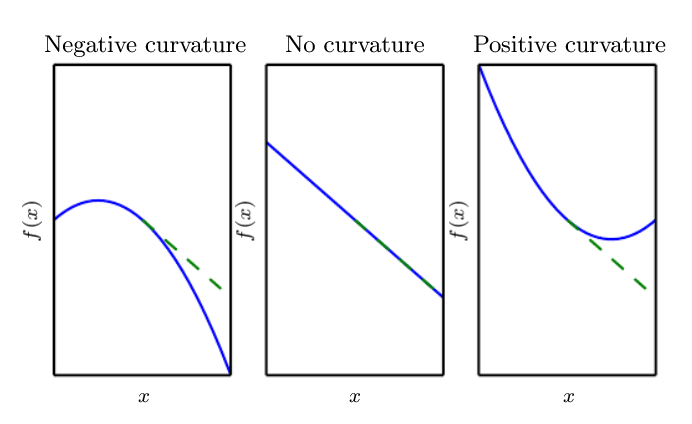
\includegraphics[width=120 mm]{images/hessian.png}
\caption{Mô tả điểm yếu của các phương pháp bậc nhất không thể phân biệt đường cong xuống (trái), mặt phẳng (giữa), đường cong lên (phải).\cite{goodfellow2016deeplearning}}
\label{fig:hessian}
\end{figure}

Do đạo hàm bậc nhất thiếu đi thông tin về độ cong bề mặt lỗi (Hình \ref{fig:hessian}), nên các phương pháp bậc nhất hay xảy ra hiện tượng dao động do hướng của gradient không trùng với hướng để đi tới cực tiểu. Phương pháp giảm độ lớn bước cập nhật thường được chọn để khắc phục hiện tượng này. Tuy nhiên, với một bước cập nhật quá nhỏ, các phương pháp bậc nhất có thể tạo hiện tượng "cực tiểu giả". Hiện tượng tạo ra từ việc hướng cho độ lỗi giảm nhiều nhất trùng với hướng có độ cong thấp, là hướng có tốc độ cập nhật rất chậm\cite{martens2010deeplv}. Các phương pháp bậc hai nhắm đến việc cải thiện điểm yếu này bằng việc sử dụng ma trận Hessian, là ma trận đạo hàm bậc hai theo từng cặp hướng, để xác định độ dài phù hợp cho từng hướng cập nhật. Tuy nhiên, các phương pháp bậc hai thường bị các điểm cực tiểu và cực đại ``thu hút'' nên dễ dàng bị mắc kẹt tại các điểm yên ngựa, tại đó vừa là cực tiểu trên chiều này nhưng là cực đại trên chiều khác. Mặt khác, việc tính toán đạo hàm bậc hai đòi hỏi nhiều chi phí tính toán và tiêu tốn bộ nhớ cấp số mũ với số lượng trọng số của mạng. Đối với các mạng nơ-ron nhiều tầng ẩn mà số lượng trọng số có thể lên đến hàng tỷ thì đây là bất khả thi. Vì vậy, một số phương pháp bậc nhất thực hiện xấp xỉ ma trận Hessian thông qua bình phương của gradient bậc nhất. Nhờ thông tin có được từ xấp xỉ ma trận Hessian, các phương pháp này sẽ có thể ``thích ứng'' tỉ lệ học cho từng trọng số trong mạng nơ-ron một cách tối ưu hon, thay vì sử dụng một tỉ lệ học chung cho tất cả trọng số như các phương pháp khác. Nhóm các phương pháp này được gọi là các phương pháp tỉ lệ học thích ứng (adaptive learning rate).

Phương pháp tỉ lệ học thích ứng có nhiều ưu điểm. Đầu tiên, phương pháp này cho phép tự động điều chỉnh tỉ lệ học tương ứng cho từng trọng số, giúp giảm số lượng siêu tham số cần phải tinh chỉnh trước quá trình huấn luyện. Thứ hai, nhờ xấp xỉ thông tin của ma trận Hessian và thích ứng tỉ lệ học cho từng trọng số, phương pháp này cho bước cập nhật tại các vùng có độ cong cao nhỏ hơn các vùng có độ cong thấp. Điều này giúp khắc phục hiện tượng dao động trong vùng rãnh hẹp để từ đó tăng nhanh tốc độ hội tụ.

Tuy nhiên, phương pháp tỉ lệ học thích ứng cũng có một số hạn chế. Thứ nhất, vì xấp xỉ thông tin từ ma trận Hessian nên phương pháp cũng gặp phải những hạn chế khi các xấp xỉ bậc hai xác định một bước nhảy có kích thước quá lớn dẫn đến hiện tượng dao động tại vùng gần cực tiểu. Thứ hai, trong quá trình thích ứng tỉ lệ học cho từng trọng số, các trọng số được xét độc lập với nhau và tương ứng với các trục. Điều này hạn chế lợi thế của thuật toán khi các hướng có độ dốc cao không tương ứng với trục trọng số.

Lấy ý tưởng từ những phương pháp trên, Diederik P. Kingma và Jimmy Lei Ba đã đề xuất một thuật toán tối ưu bậc nhất cho mạng nơ-ron nhiều tầng ẩn với tốc độ cao hơn so với hầu hết những thuật toán trước đó\cite{kingma2014adam}. Công trình này, ``Adam, A Method for Stochastic Optimization'', được công bố tại hội nghị ``International Conference on Learning Representation 2015''. Ý tưởng của thuật toán là kết hợp hai hướng tiếp cận trước đó: (1) sử dụng quán tính để tăng tốc và giảm dao động, và (2) thích ứng tỉ lệ học cho từng trọng số. Thuật toán Adam sử dụng trung bình chạy để tích tụ quán tính kết hợp với phương pháp xấp xỉ ma trận Hessian của phương pháp tỉ lệ học thích ứng cho phép Adam hoạt động tốt trong trường hợp dữ liệu thưa. Ngoài ra, Adam còn thực hiện bias-correction giúp thuật toán không bị ``bias'' về giá trị khởi tạo cho phép thực hiện các bước cập nhật tốt hơn ngay những bước đầu tiên. Nhờ sự kết hợp này, Adam kế thừa được nhiều ưu điểm, đồng thời khắc phục những hạn chế của các hướng tiếp cận trên khi có thể tăng giảm độ dài bước cập nhật tùy theo điều kiện bề mặt lỗi. Trong khóa luận này, chúng tôi tìm hiểu và cài đặt lại thuật toán Adam cùng với các thuật toán liên quan. Chúng tôi cũng thực hiện thêm các thí nghiệm nhằm phân tích và làm rõ cách mỗi phương pháp giải quyết các khó khăn trong việc huấn luyện mạng nơ-ron nhiều tầng ẩn. Ngoài ra, chúng tôi cũng sử dụng tính toán song song trên GPU để tăng tốc độ xử lí cho các thí nghiệm.

Phần còn lại của khóa luận được trình bày như sau:

\begin{itemize}
	\item Chương 2 giới thiệu sơ lược về mạng nơ-ron nhiều tầng ẩn và quá trình huấn luyện, cũng như nguyên lý của thuật toán Gradient Descent.
	\item Chương 3 trình bày về thuật toán Adam và các thuật toán nền tảng. Chương này là phần chính của khóa luận.
	\item Chương 4 trình bày về các thí nghiệm về nguyên lý cũng như thực tiễn để phân tích các tính chất của thuật toán Adam.
	\item Cuối cùng, chương 5 trình bày kết luận và hướng phát triển.
\end{itemize}
